\apendice{Especificación de Requisitos}

\section{Introducción}
Este anexo recoge los distintos requisitos del proyecto.
Está organizado en dos apartados: 
\begin{itemize}
    \item Catálogo de Requisitos: Recoge los requisitos funcionales y no funcionales del proyecto.
    \item Casos de Uso: Detallan la visión del proyecto y permiten realizar una implementación de la aplicación. 
\end{itemize}


\section{Objetivos generales}
\begin{enumerate}
    \item
        Diseñar e implementar un servicio web que extienda la capacidades de un servicio ya existente.
    \item 
        Diseñar e implementar una arquitectura que interconecte múltiples servicios.
    \item
        Diseñar e implementar un servicio que permita analizar y recomendar canciones a partir de un fichero de audio musical.
\end{enumerate}

\section{Catálogo de Requisitos}

\subsection{Requisitos Funcionales}\label{requisitos-funcionales}
\begin{itemize}
\tightlist

    \item
        \textbf{RF-1 Gestión de Biblioteca:} Se requiere que la web sea capaz de mostrar la biblioteca de música personal del usuario.
        \begin{itemize}
           \tightlist
           
            \item
                \textbf{RF-1.1 Listar Biblioteca:} Se requiere que el usuario pueda visualizar su biblioteca de usuario
                \begin{itemize}
                    \item
                        \textbf{RF-1.1.1 Filtrar Vista:} Se requiere que el usuario pueda filtrar la vista de su biblioteca mediante filtros avanzados.
                    \item
                        \textbf{RF-1.1.2 Seleccionar Vista:} Se requiere que el usuario pueda marcar como seleccionados los elementos filtrados.
                    \item
                        \textbf{RF-1.1.3 Ordenar Vista:} Se requiere que el usuario pueda ordenar la vista actual a partir de parámetros.
                    \item
                        \textbf{RF-1.1.3 Detallar Canción:} Se requiere que el usuario pueda ver detalles de cualquier item de la vista. 
                \end{itemize}
                
            \item
                \textbf{RF-1.2 Crear Playlist:} Se requiere que el usuario pueda crear playlists a partir de una selección de canciones.   
                \begin{itemize}
                    \item 
                        \textbf{RF-1.2.1 Configurar Playlist:} Se requiere que el usuario pueda escoger el título, descripción y opciones de privacidad de cada playlist.
                    \item 
                        \textbf{RF-1.2.2 Dividir Playlist:} Se requiere que el usuario pueda dividir una playlist en múltiples playlists.
                    \item
                        \texbf{RF-1.2.3 Expandir con Recomendaciones}: Se requeire qu el usuario pueda añadir a la playlist recomendaciones. 
                \end{itemize}
                
            \item
                \textbf{RF-1.3 Ampliar Playlists:} Se requiere que el usuario pueda ampliar sus playlists ya creadas a partir de una selección de canciones.
                \begin{itemize}
                    \item
                        \textbf{RF-1.3.1 Buscar Playlist:} Se requiere que el usuario pueda seleccionar su playlist a partir de un listado.
                    \item
                        \textbf{RF-1.3.2 Detallar Playlist:} Se requiere que el usuario pueda ver los detalles de una playlist.
                \end{itemize}
                
            \item
                \textbf{RF-1.4 Detallar Playlist:} Se requiere que el usuario pueda ver los detalles de su playlist.
        \end{itemize}
    

        
    \item  
        \textbf{RF-2 Gestión de Álbumes:} Se requiere que la web sea capaz de mostrar los álbumes del usuario.
        \begin{itemize}
            \item 
                \textbf{RF-2.1 Listar Álbumes:} Se requiere que el usuario pueda visualizar sus álbumes.
                \begin{itemize}
                    \item 
                        \textbf{RF-2.1.1 Álbumes Favoritos:} Se requiere que el usuario pueda visualizar sus álbumes marcados como favoritos.
                    \item 
                        \textbf{RF-2.1.2 Álbumes Etiquetados:} Se requiere que el usuario pueda visualizar sus álbumes etiquetados.
                        
                    \item
                        \textbf{RF-2.1.3 Filtrar Vista:} Se requiere que el usuario pueda filtrar la vista actual de sus álbumes mediante filtros avanzados.
                    \item
                        \textbf{RF-2.1.4 Ordenar Vista:} Se requiere que el usuario pueda ordenar la vista actual a partir de parámetros.
                    \item
                        \textbf{RF-2.1.5 Detallar Álbum:} Se requiere que el usuario pueda ver detalles de cualquier álbum en la vista. 
                \end{itemize}
                
            \item 
                \textbf{RF-2.2 Buscar Álbumes:} Se requiere que el usuario pueda visualizar álbumes a partir de una cadena.
            \item
                \textbf{RF-2.3 Gestionar Álbumes Favoritos:} Se requiere que el usuario pueda marcar o desmarcar cualquier álbum como favorito.
            \item
                \textbf{RF-2.4 Etiquetar Álbumes:} Se requiere que el usuario Añadir etiquetas a cualquier álbum.
                \begin{itemize}
                    \item 
                    \textbf{RF-2.4.1 Etiquetas Personalizadas:} Se requiere que el usuario pueda crear sus propias etiquetas.
                \end{itemize}
        \end{itemize}

    \item
        \textbf{RF-3 Detallar Elementos:} Se requiere que el usuario pueda ver detalles de un álbum, playlist o seleccionado por el usuario.
            \begin{itemize}
                \item 
                \textbf{RF-3.1 Detallar Canción:} Se requiere que el usuario pueda ver detalles de una canción específica.
                    \begin{itemize}
                        \item 
                            \textbf{RF-3.1.1 Previsualizar Canción:} Se requiere que el usuario pueda escuchar un fragmento de la canción.
                        \item
                            \textbf{RF-3.1.2 Analizar Canción:} Se requiere que el usuario pueda obtener detalles especiales a partir de un análisis de un fragmento de la canción.
                        \item
                            \textbf{RF-3.1.3 Reproducir Canción:} Se requiere que el usuario pueda reproducir o añadir a la cola una canción en un cliente de Spotify.
                        \item
                            \textbf{RF-3.1.4 Detallar Álbum:} Se requiere que el usuario obtenga los detalles del álbum al que pertenece dicha canción.

                    \end{itemize}
                    
                \item 
                \textbf{RF-3.2 Detallar Álbum:} Se requiere que el usuario pueda ver detalles de un álbum específico.
                    \begin{itemize}
                        \item 
                            \textbf{RF-3.2.1 Gestionar Etiquetas:} Se requiere que el usuario pueda visualizar o gestionar las etiquetas de un álbum
                        \item 
                            \textbf{RF-3.2.2 Conocer Estadísticas:} Se requiere que el usuario pueda ver las estadísticas del álbum mediante LastFM.
                        \item 
                            \textbf{RF-3.2.3 Reproducir Álbum:} Se requiere que el usuario pueda reproducir el álbum en un cliente Spotify.                 
                        \item 
                            \textbf{RF-3.2.3 Detallar Artistas:} Se requiere que el usuario pueda conocer los detalles de los artistas que han participado en el álbum.
                    \end{itemize}
                \item
                    \textbf{RF-3.3 Detallar Playlist:} Se requiere que el usuario pueda conocer los detalles de una playlist.
                    \begin{itemize}
                        \item \textbf{RF-3.3.1 Detallar Canciones} Se requiere que el usuario pueda explorar las canciones de una playlist.
                    \end{itemize}             
                \item
                    \textbf{RF-3.4 Detallar Artistas:} Se requiere que el usuario pueda conocer los detalles de un artista en específico.
                    \begin{itemize}
                        \item \textbf{RF-3.4.1 Géneros Musicales} Se requiere que el usuario pueda conocer los géneros musicales de un artista. 
                    \end{itemize}
            \end{itemize}

    \item
        \textbf{RF-4 Gestión de Tema:} Se requiere que el usuario pueda cambiar el tema actual en cualquier punto de la web.
            \begin{itemize}
                \item 
                \textbf{RF-4.1 Tema Persistente:} Se requiere que el tema seleccionado se mantenga entre sesiones. 
            \end{itemize}
            
    \item
        \textbf{RF-5 Gestión de Sesión:} Se requiere que el usuario tenga el control de la sesión actual.
        \begin{itemize}
            \item
                \textbf{RF-5.1 Cerrar Sesión:} Se requiere que el usuario pueda cerrar su sesión desde la web.
                \begin{itemize}
                    \item
                    \textbf{RF-5.1.1 Limpieza de Sesión:} Se requiere que todos los datos locales sean borrados al cerrar sesión.
                \end{itemize}
            \item
                \textbf{RF-5.2 Limpiar Datos Locales:} Se requiere que los datos locales puedan borrarse desde la web.
        \end{itemize}
    
    \item
        \textbf{RF-5 Estadísticas:} Se requiere que el usuario pueda visualizar las estadísticas relacionadas con su cuenta.
        \begin{itemize}
            \item \textbf{RF-5.1 Listar Canciones}: Se requiere que el usuario pueda conocer sus canciones más escuchadas en diversos periodos de tiempo.
            \item \textbf{RF-5.2 Listar Artistas}: Se requiere que el usuario pueda conocer sus artistas más escuchadas en diversos periodos de tiempo.
        \end{itemize}
    
    \item
        \textbf{RF-6 Cachear Peticiones:} Se requiere que la aplicación realice el mínimo número de peticiones a la API para no sobrepasar los límites.
            \begin{itemize}
                \item \textbf{RF-6.1 Cachear Canciones:} Se requiere que los datos de las canciones se almacenen de forma local.
                \item \textbf{RF-6.2 Cachear Artistas:} Se requiere que los datos de los artistas se almacenen de forma local.
                \item \textbf{RF-6.3 Cachear Álbumes:} Se requiere que los datos de los álbumes se almacenen de forma local.
                \item \textbf{RF-6.4 Refrescar Caché:} Se requiere que los distintos datos almacenados puedan actualizarse para evitar inconsistencias.
            \end{itemize}
    \item
        \textbf{RF-7 Analizar Canciones:} Se requiere que el usuario pueda conocer detalles de cada una de las canciones a partir de un fragmento de la canción.
\end{itemize}

\subsection{Requisitos no Funcionales}\label{requisitos-no-funcionales}
\begin{itemize}
    \item \textbf{RNF-1 Diseño Responsive:} Se requiere un diseño "responsive" para poder utilizarla en dispositivos con distintos tamaños de pantalla o relaciones de aspecto sin perder información.
    \item \textbf{RNF-2 Minimizar Peticiones:} Se requiere minimizar el número de peticiones posibles a las  distintas APIs para evitar alcanzar los límites de cada API. 
    \item \textbf{RNF-3 Internacionalización:} Se requiere que la web esté disponible en, al menos, dos idiomas.
    
    \item\textbf{RNF-4 Compatibilidad:} Se requiere que la web sea funcional a lo largo de los motores webs más utilizados (Chromium, Firefox y Apple Webkit).
    \item\textbf{RNF-5 Carga Diferida:} Se requiere que la web evite cargar un exceso de datos si el usuario no va a necesitarlos, por ejemplo aplicando el patón de Carga Diferida para paginar la carga de recursos remotos. 
    \item\textbf{RNF-6 Accesibilidad:} Se requiere que la web cumpla con el mayor número de recomendaciones posible de Web Content Accessibility Guidelines (WCAG) 2.1
    \item\textbf{RNF-7 Rendimiento y Buenas Prácticas:} Se requiere que la web funcione correctamente en dispositivos móviles y en escritorio, minimizando el tamaño de la aplicación para acelerar las cargas de JavaScript y evitar las esperas en el navegador.
    \item\textbf{RNF-8 Seguridad:} Se requiere que la web sea segura, utilizando TSL o SSL.
    \item\textbf{RNF-9 Privacidad:} Se requiere almacenar el mínimo de información que puede identificar a un usuario para mejorar la privacidad de los datos. 
\end{itemize}
\clearpage

\section{Especificación de requisitos}
Esta sección contiene el diagrama de casos de uso y la especificación individual de los casos de uso más importantes. 

\subsection{Actores}
Únicamente hay un actor, el \texbf{usuario} final. 

\subsection{Diagrama de Casos de Uso}
El diagrama de casos de uso únicamente contiene un actor, y está dividido en dos imágenes.

\begin{figure}[H]
    \begin{center}
        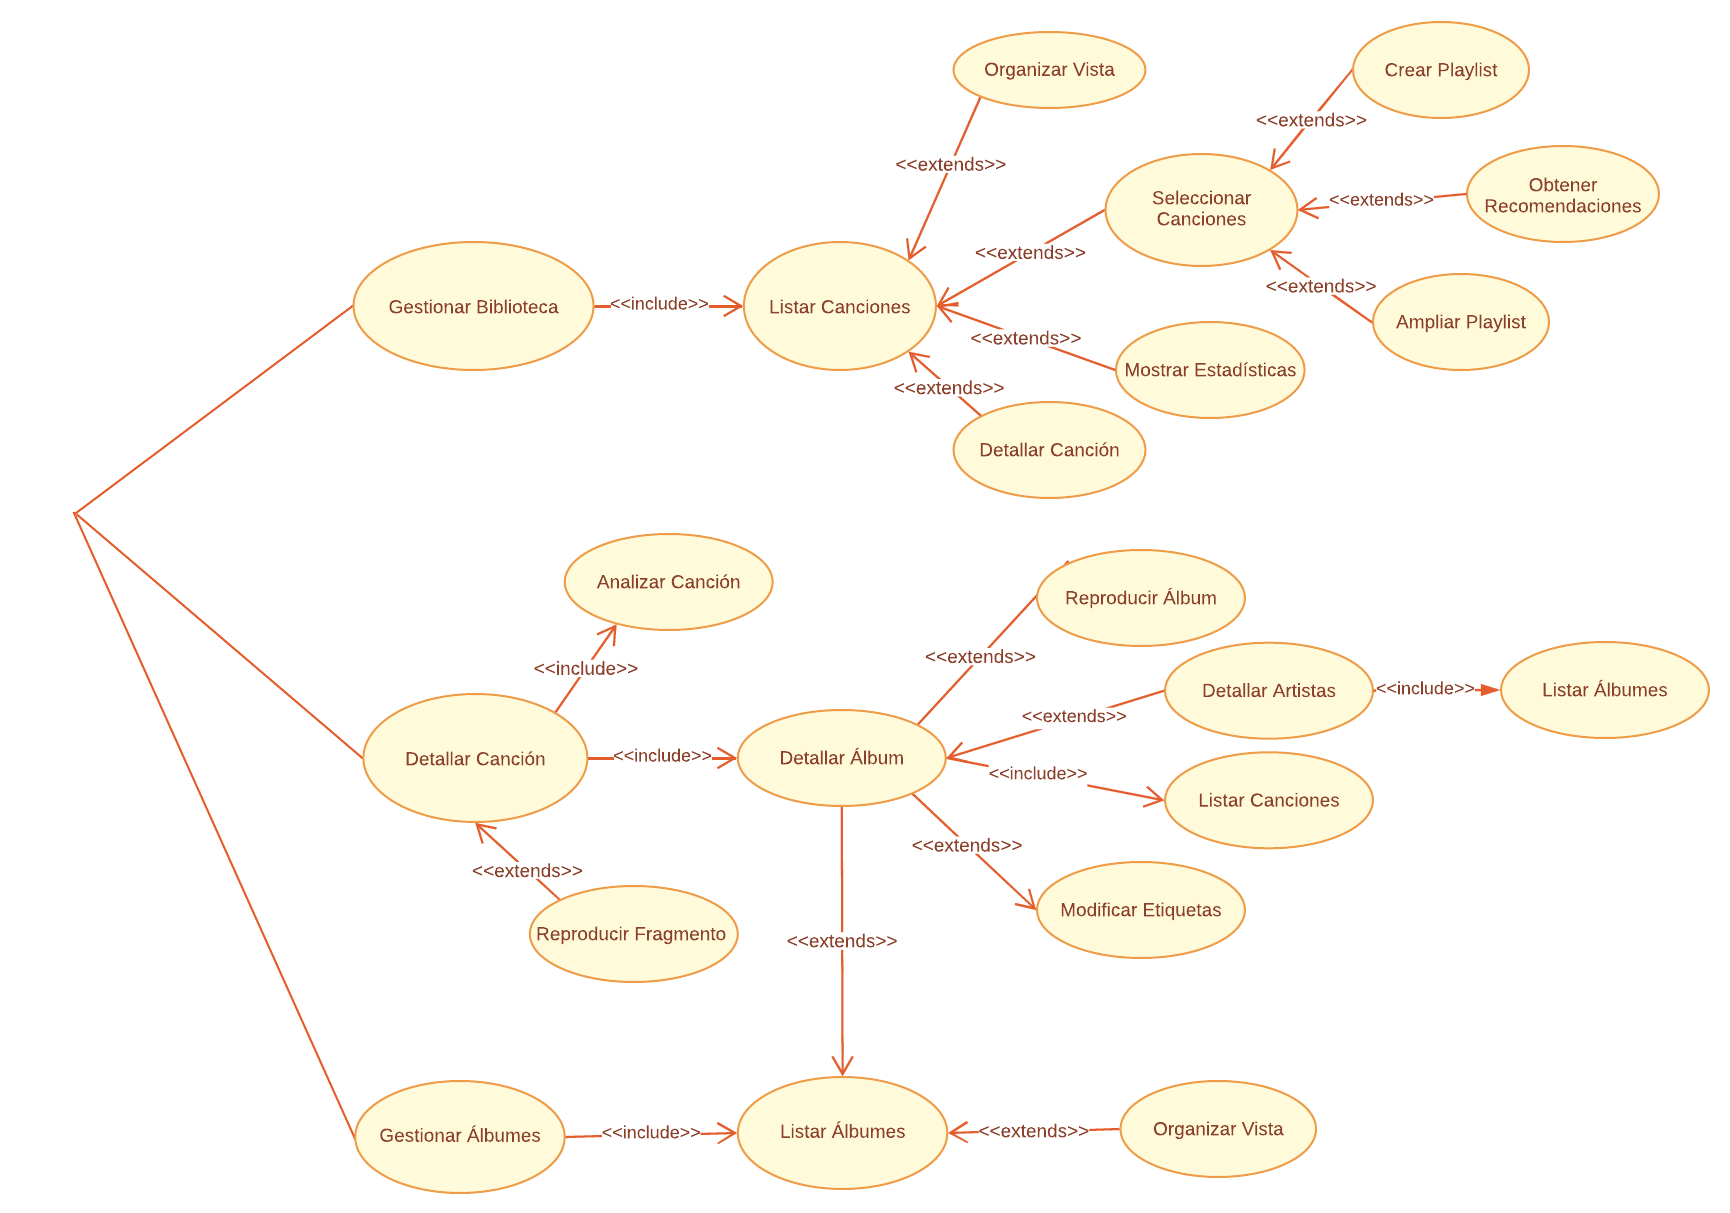
\includegraphics[]{img/B/CU_1.png}
        \caption{Casos de Uso - Parte 1}
        \label{fig:CU_1}
    \end{center}

\end{figure}

\begin{figure}[H]
    \begin{center}
        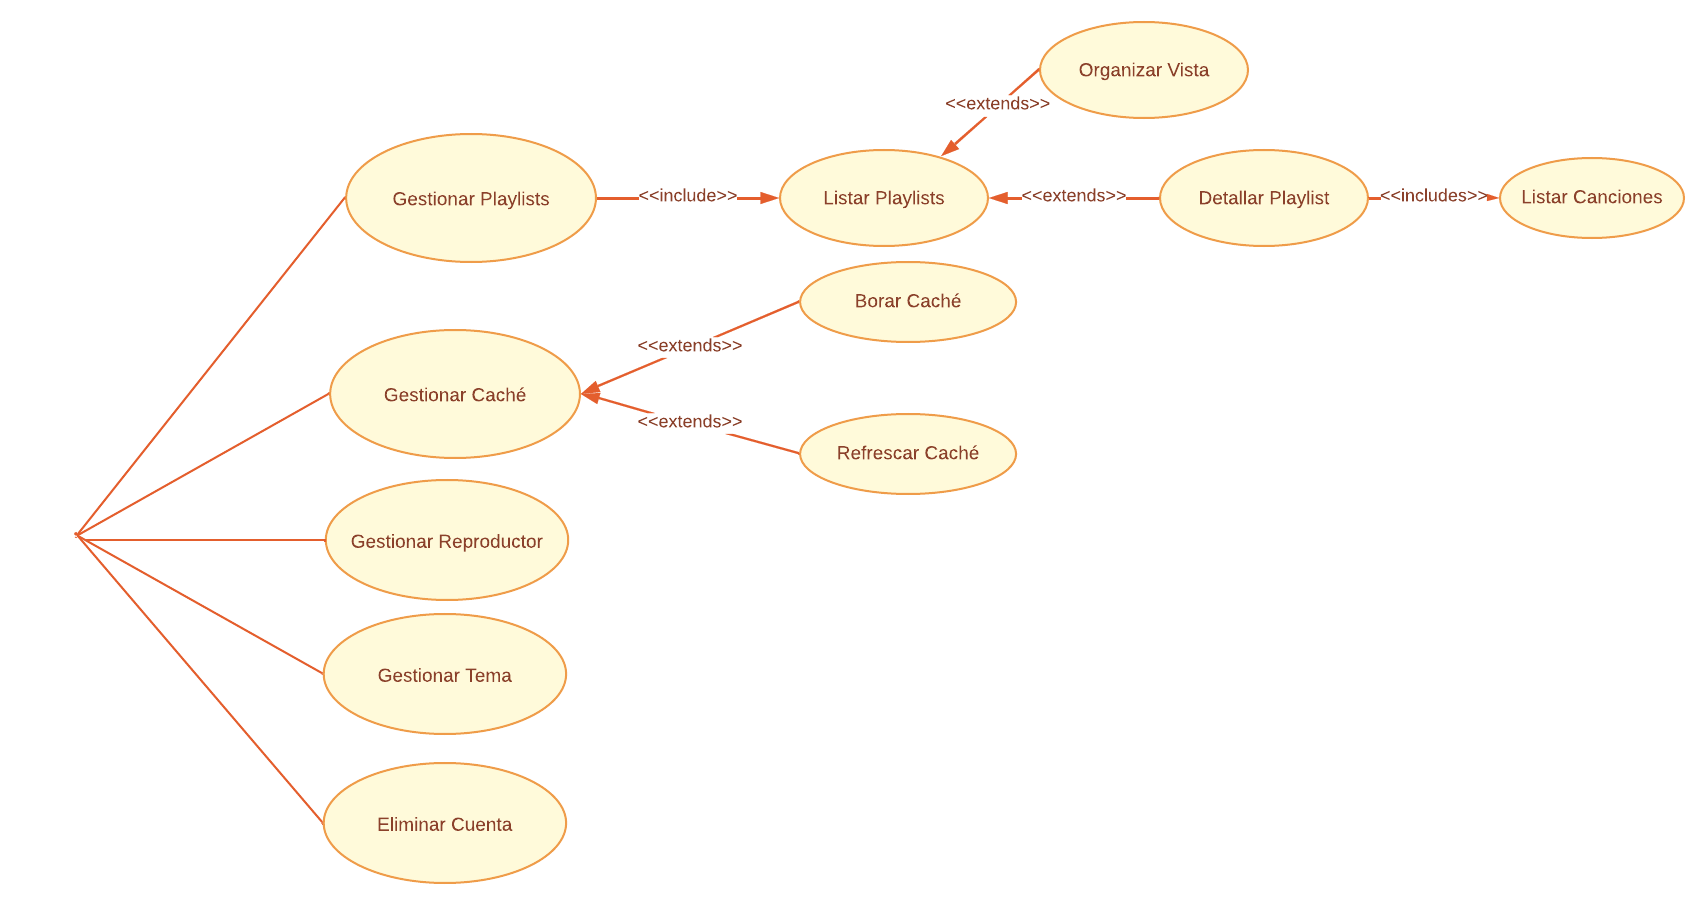
\includegraphics[]{img/B/CU_2.png}
        \caption{Casos de Uso - Parte 2}
        \label{fig:CU_2}
    \end{center}

\end{figure}
\clearpage


\subsection{Casos de Uso}

En este apartado se van a detallar los distintos casos de uso. 

\begin{table}[H]
    \centering
    \begin{tabular}{r|p{0.6\textwidth}}
    \hline
    \textbf{CU-01}         & \textbf{Gestionar Tema}                                 \\ \hline
    \textbf{Versión}       & 1.0                                                     \\
    \textbf{Autor}         & Jorge Ruiz Gómez                                        \\
    \textbf{Requisitos}    & RF-4                                         \\
    \textbf{Descripción}   & Permite al usuario cambiar el tema general de la página \\ \hline
    \textbf{Precondición}  & Ninguna                                                 \\
    \textbf{Acciones}      &    \begin{itemize}
                                    \item El Usuario entra en la página.
                                    \item La web carga el tema almacenado.
                                    \item El usuario pulsa el botón de cambio de tema.
                                    \item El Tema se alterna.
                                    \item La selección del tema se almacena de forma local.
                                \end{itemize}\\
                                                                              
    \textbf{Postcondición} & El tema ha cambiado                                     \\
    \textbf{Excepciones}   & Ninguna                                                 \\
    \textbf{Importancia}   & Baja                                                    \\ \hline
    \end{tabular}
    \caption{CU-01}
    \label{tab:my-table}
\end{table}


\begin{table}[H]
    \centering
    \begin{tabular}{r|p{0.6\textwidth}}
    \hline
    \textbf{CU-02}         & \textbf{Gestionar Estadísticas}                                 \\ \hline
    \textbf{Versión}       & 1.0                                                     \\
    \textbf{Autor}         & Jorge Ruiz Gómez                                        \\
    \textbf{Requisitos}    & RF-5                                         \\
    \textbf{Descripción}   & Permite al usuario conocer de manera visual estadísticas calculadas a partir de la vista de canciones actual. Estas estadísticas incluyen los géneros y estados de ánimo favoritos, evolución de géneros musicales o gráficos con la actividad de la cuenta del usuario.  \\ \hline
    \textbf{Precondición}  & El usuario ha iniciado sesión.                                              \\
    \textbf{Acciones}      &    \begin{itemize}
                                    \item El Usuario abre una vista de canciones.
                                    \item El usuario espera a que se carguen las canciones.
                                    
                                    \item El usuario pulsa el botón "Estadísticas".
                                    \item El usuario visualiza las estadísticas de la vista actual.
    
                                \end{itemize}\\
                                                                              
    \textbf{Postcondición} & Ninguna                              \\
    \textbf{Excepciones}   & Ninguna                                                 \\
    \textbf{Importancia}   & Baja                                                    \\ \hline
    \end{tabular}
    \caption{CU-02}
    \label{tab:CUT-02}
\end{table}

\begin{table}[H]
    \centering
    \begin{tabular}{r|p{0.6\textwidth}}
    \hline
    \textbf{CU-03}         & \textbf{Gestionar Caché}                                 \\ \hline
    \textbf{Versión}       & 1.0                                                     \\
    \textbf{Autor}         & Jorge Ruiz Gómez                                        \\
    \textbf{Requisitos}    & RF-6.4 y RF-5.2                                       \\
    \textbf{Descripción}   & Permite al usuario tener control sobre la caché local \\ \hline
    \textbf{Precondición}  & El usuario ha iniciado sesión                                                 \\
    \textbf{Acciones}      &    \begin{itemize}
                                    \item El Usuario entra en la página.
                                    \item El usuario va a a la sección de opciones.
                                    \item El usuario accede al apartado $Caché Local$.
                                    \item El usuario selecciona entre $Borrar$ o $Refrescar Caché$. 
                                \end{itemize}\\
                                                                              
    \textbf{Postcondición} & Aparece una notificación con el estado de la operación.\\
    \textbf{Excepciones}   & Ninguna                                                 \\
    \textbf{Importancia}   & Baja                                                    \\ \hline
    \end{tabular}
    \caption{CU-03}
    \label{tab:CUT-03}
\end{table}

\begin{table}[H]
    \centering
    \begin{tabular}{r|p{0.6\textwidth}}
    \hline
    \textbf{CU-04}         & \textbf{Eliminar Cuenta}                                 \\ \hline
    \textbf{Versión}       & 1.0                                                     \\
    \textbf{Autor}         & Jorge Ruiz Gómez                                        \\
    \textbf{Requisitos}    & RNF-4                                         \\
    \textbf{Descripción}   & Permite al usuario eliminar todos los datos asociados con su usuario de Spotify en la base de datos de SpotMyFM. \\ \hline
    \textbf{Precondición}  & El usuario ha iniciado sesión                                                 \\
    \textbf{Acciones}      &    \begin{itemize}
                                    \item El Usuario entra en la página.
                                    \item El usuario va a a la sección de $opciones$.
                                    \item El usuario accede al apartado $Cuenta$.
                                    \item El usuario selecciona $Eliminar Cuenta$. 
                                    \item El usuario confirma la operación. 
                                \end{itemize}\\
                                                                              
    \textbf{Postcondición} & Aparece una notificación con el estado de la operación.\\
    \textbf{Excepciones}   & Ninguna                                                 \\
    \textbf{Importancia}   & Media                                                    \\ \hline
    \end{tabular}
    \caption{CU-04}
    \label{tab:CUT-04}
\end{table}


\begin{table}[H]
    \centering
    \begin{tabular}{r|p{0.6\textwidth}}
    \hline
    \textbf{CU-05, CU-06, CU-07}         & \textbf{Gestionar Biblioteca/Albumes/Playlists}                                 \\ \hline
    \textbf{Versión}       & 1.0                                                     \\
    \textbf{Autor}         & Jorge Ruiz Gómez                                        \\
    \textbf{Requisitos}    & RF-1, F-1.3, RF-1.4, RF-2                                         \\
    \textbf{Descripción}   & Permite al usuario explorar su biblioteca de canciones / álbumes / playlists / artistas desde la aplicación, con funcionalidades extendidas. \\ \hline
    \textbf{Precondición}  & El usuario ha iniciado sesión  \\
    \textbf{Acciones}      &    \begin{itemize}
                                    \item El Usuario entra en la página.
                                    \item El usuario va a a la sección $Gestionar Biblioteca$ desde la barra de navegación.
                                    \item El usuario descarga su biblioteca localmente.
                                \end{itemize}\\
                                                                              
    \textbf{Postcondición} & Se elimina el bloqueo y están disponibles todas las canciones del usuario \\
    \textbf{Excepciones}   & Ninguna                                                 \\
    \textbf{Importancia}   & Alta                                                   \\ \hline
    \end{tabular}
    \caption{CU-05, CU-06 y CU-07}
    \label{tab:CUT-05}
\end{table}

\begin{table}[H]
    \centering
    \begin{tabular}{r|p{0.6\textwidth}}
    \hline
    \textbf{CU-08}         & \textbf{Organizar Vista}                                 \\ \hline
    \textbf{Versión}       & 1.0                                                     \\
    \textbf{Autor}         & Jorge Ruiz Gómez                                        \\
    \textbf{Requisitos}    & RF-1.1.1, RF-1.1.3, RF-2.1.3, RF-2.1.4                                         \\
    \textbf{Descripción}   & Permite al usuario filtrar u ordenar una vista. \\ \hline
    \textbf{Precondición}  & El usuario ha iniciado sesión. Estamos trabajando con una vista de canciones, álbumes, artistas o playlists.  \\
    \textbf{Acciones}      &    \begin{itemize}
                                    \item El usuario abre una vista.
                                    \item El usuario pulsa sobre un desplegable con el que puede seleccionar un atributo por el que ordenar.
                                    \item El usuario escoge un atributo y se refresca la vista con el nuevo orden.
                                    \item El usuario escribe en un campo. 
                                    \item La vista muestra únicamente los elementos cuyos atributos coinciden con los valores del campo.
                                \end{itemize}\\
                                                                              
    \textbf{Postcondición} & Ninguna \\
    \textbf{Excepciones}   & Ninguna                                                 \\
    \textbf{Importancia}   & Baja                                                   \\ \hline
    \end{tabular}
    \caption{CU-08}
    \label{tab:CUT-08}
\end{table}

\begin{table}[H]
    \centering
    \begin{tabular}{r|p{0.6\textwidth}}
    \hline
    \textbf{CU-09}  & \textbf{Listar}                                 \\ \hline
    \textbf{Versión}       & 1.0                                                     \\
    \textbf{Autor}         & Jorge Ruiz Gómez                                        \\
    \textbf{Requisitos}    & RF-1.1, RF-1.3.2 RF-2.1, RF-5.1, RF-5.2                                         \\
    \textbf{Descripción}   & Permite al usuario listar todas las canciones/artistas/álbumes/playlist. \\ \hline
    \textbf{Precondición}  & El usuario ha iniciado sesión.\\
    \textbf{Acciones}      &    \begin{itemize}
                                    \item El usuario abre una vista a partir de un gestor u otra biblioteca anidada.
                                    \item Si se realiza desde un móvil aparece una lista con canciones. Si no, aparecen tarjetas con la carátula del álbum  de cada canción en grande.
                                    \item Cada elemento en la lista se puede detallar. Al detallar un elemento se abre un Modal con los detalles.
                                    
                                    \item\texbf{Listar Canciones}: Se puede acceder a esta vista a partir de la gestión de la biblioteca \ref{tab:CUT-05}, así como los detalles de un álbum (canciones que componen un álbum) o los detalles de una playlist (canciones que componente una playlist)
                                
                                \item\texbf{Listar Álbumes}: Se puede acceder a esta vista a partir de los detalles de un artista (álbumes que ha publicado un artista) y la gestión de los álbumes de usuario \ref{tab:CUT-05}
                                
                                \item\texbf{Listar Playlists}: Se puede acceder a esta vista desde el gestor de playlists. \ref{tab:CUT-05}
                                
                                \item\texbf{Listar Artistas}: Se puede acceder a esta vista desde los detalles de un álbum.
                                \end{itemize}\\
                                

    \textbf{Postcondición} & Ninguna \\
    \textbf{Excepciones}   & Hay un fallo en la comunicación con Spotify.                                                 \\
    \textbf{Importancia}   & Alta                                                    \\ \hline
    \end{tabular}
    \caption{CU-09}
    \label{tab:CUT-09}
\end{table}


\begin{table}[H]
    \centering
    \begin{tabular}{r|p{0.6\textwidth}}
    \hline
    \textbf{CU-10, CU-10.1, CU-10.2}  & \textbf{Seleccionar Canciones}                                 \\ \hline
    \textbf{Versión}       & 1.0                                                     \\
    \textbf{Autor}         & Jorge Ruiz Gómez                                        \\
    \textbf{Requisitos}    & RF-1.2                                       \\
    \textbf{Descripción}   & Permite al usuario seleccionar una serie de canciones que pueden ser utilizada para la creación o ampliación de playlists. \\ \hline
    \textbf{Precondición}  & El usuario ha iniciado sesión. Estamos trabajando con una vista de canciones. \ref{tab:CUT-09}  \\
    \textbf{Acciones}      &    \begin{itemize}
                                    \item El usuario abre una con canciones.
                                    \item El usuario pulsa sobre el botón $Añadir a la Playlist$.
                                    \item El botón cambia su etiqueta a $Eliminar de la Playlist$
                                    \item Un menú para configurar la playlist es visible.


                                            \textbf{Ampliar Playlist}
                                            \begin{itemize}
                                                \item El usuario selecciona una playlist de la lista.
                                                \item El usuario añade las canciones a la playlist.
                                            \end{itemize}
  
                                            \textbf{Crear Playlist}
                                            \begin{itemize}
                                                \item El usuario introduce el nombre de la playlist
                                                \item El usuario introduce el numero de playlists que desea generar (un número mayor que 0)
                                                \item El usuario pulsa sobre el botón crear.
                                            \end{itemize}

                                \end{itemize}\\
                                                                              
    \textbf{Postcondición} & No hay canciones seleccionadas y aparece un mensaje confirmado el estado de la creación. \\
    \textbf{Excepciones}   & Hay un fallo con la API de Spotify.                                                 \\
    \textbf{Importancia}   & Media                                                    \\ \hline
    \end{tabular}
    \caption{CU-10}
    \label{tab:CUT-10}
\end{table}




\begin{table}[H]
    \centering
    \begin{tabular}{r|p{0.6\textwidth}}
    \hline
    \textbf{CU-10.3}  & \textbf{Recomendar Canciones}                                 \\ \hline
    \textbf{Versión}       & 1.0                                                     \\
    \textbf{Autor}         & Jorge Ruiz Gómez                                        \\
    \textbf{Requisitos}    & RNF-1.2.3                                         \\
    \textbf{Descripción}   & Permite al usuario conseguir una lista con canciones similares. \\ \hline
    \textbf{Precondición}  & El usuario ha seleccionado una o más canciones\\
    \textbf{Acciones}      &    \begin{itemize}
                                    \item El usuario pulsa sobre el botón $Recomendaciones$.
                                    \item Se abre una nueva vista con nuevas canciones.
                                    \item El usuario selecciona una o varias canciones.
                                    \item El usuario vuelve a lista anterior.
                                \end{itemize}\\
                                                                              
    \textbf{Postcondición} & Se han añadido las nuevas canciones a la vista original. \\
    \textbf{Excepciones}   & Hay un fallo en la comunicación con el servidor de canciones.                                                 \\
    \textbf{Importancia}   & Baja                                                    \\ \hline
    \end{tabular}
    \caption{CU-10.3}
    \label{tab:CUT-10.3}
\end{table}


\begin{table}[H]
    \centering
    \begin{tabular}{r|p{0.6\textwidth}}
    \hline
    \textbf{CU-11}  & \textbf{Modificar Etiquetas}                                 \\ \hline
    \textbf{Versión}       & 1.0                                                     \\
    \textbf{Autor}         & Jorge Ruiz Gómez                                        \\
    \textbf{Requisitos}    & RF-2.4                                        \\
    \textbf{Descripción}   & Permite al usuario modificar las etiquetas de un álbum. \\ \hline
    \textbf{Precondición}  & El usuario ha detallado un álbum.\\
    \textbf{Acciones}      &    \begin{itemize}
                                    \item El usuario pulsa sobre el botón $Editar Etiqutetas$.
                                    \item Se abre una nueva vista con una lista de etiquetas y un campo de texto.
                                    \item El usuario pulsa sobre una etiqueta para eliminarla.
                                    \item El usuario introduce una nueva etiqueta desde el campo de texto.
                                    \item El usuario guarda los cambios. 
                                \end{itemize}\\
                                                                              
    \textbf{Postcondición} & Se ha notificado el estado de la operación. \\
    \textbf{Excepciones}   & Hay un fallo en la comunicación con el servidor/base de datos.                                                 \\
    \textbf{Importancia}   & Baja                                                    \\ \hline
    \end{tabular}
    \caption{CU-11}
    \label{tab:CUT-11}
\end{table}

\begin{table}[H]
    \centering
    \begin{tabular}{r|p{0.6\textwidth}}
    \hline
    \textbf{CU-12}  & \textbf{Gestionar Reproductor}                                 \\ \hline
    \textbf{Versión}       & 1.0                                                     \\
    \textbf{Autor}         & Jorge Ruiz Gómez                                        \\
    \textbf{Requisitos}    & RF-3.1.4, RD-3.2.3                                        \\
    \textbf{Descripción}   & Permite al usuario controlar la canción que está sonando \\ \hline
    \textbf{Precondición}  & El usuario tiene una sesión activa de Spotify.\\
    \textbf{Acciones}      &    \begin{itemize}
                                    \item El usuario pulsa sobre el botón Reproducir Canción / Álbum.
                                    \item Se modifica la canción actual.
                                    \item El usuario decide si desea Pausar, Avanzar o Retroceder la cola de canciones.
                                \end{itemize}\\
                                                                              
    \textbf{Postcondición} & Se ha notificado el estado de la operación. \\
    \textbf{Excepciones}   & Hay un fallo en la comunicación con Spotify.                                                 \\
    \textbf{Importancia}   & Baja                                                    \\ \hline
    \end{tabular}
    \caption{CU-12}
    \label{tab:CUT-12}
\end{table}


\begin{table}[H]
    \centering
    \begin{tabular}{r|p{0.6\textwidth}}
    \hline
    \textbf{CU-13}  & \textbf{Detallar Canción}                                 \\ \hline
    \textbf{Versión}       & 1.0                                                     \\
    \textbf{Autor}         & Jorge Ruiz Gómez                                        \\
    \textbf{Requisitos}    & RF-3.1                                         \\
    \textbf{Descripción}   & Permite al usuario visualizar todos los atributos de una canción. Esta vista incluye datos 
    como el número de reproducciones de la canción, botón de reproducción, géneros, subgéneros y estados de ánimo\footnote{Resultados del análisis}. Además, contiene todos los detalles del álbum.
    \\ \hline
    \textbf{Precondición}  & El usuario tiene una sesión activa de Spotify y está en una lista de canciones.\\
    \textbf{Acciones}      &    \begin{itemize}
                                    \item El usuario pulsa sobre el botón (+)
                                    \item Se abre un modal con los detalles.
                                \end{itemize}\\
                                                                              
    \textbf{Postcondición} & Se ha notificado el estado de la operación. \\
    \textbf{Excepciones}   & Hay un fallo en la comunicación con Spotify.                                                 \\
    \textbf{Importancia}   & Alta                                                   \\ \hline
    \end{tabular}
    \caption{CU-13}
    \label{tab:CUT-13}
\end{table}


\begin{table}[H]
    \centering
    \begin{tabular}{r|p{0.6\textwidth}}
    \hline
    \textbf{CU-14}  & \textbf{Detallar Álbum}                                 \\ \hline
    \textbf{Versión}       & 1.0                                                     \\
    \textbf{Autor}         & Jorge Ruiz Gómez                                        \\
    \textbf{Requisitos}    & RF-3.2                                         \\
    \textbf{Descripción}   & Permite al usuario visualizar todos los atributos de un álbum. Esta vista incluye una pequeña descripción del álbum, sus etiquetas de usuario, un botón para poder editar las etiquetas de usuario y una lista con todos los artistas \ref{tab:CUT-09} que han participado en el álbum. Además, se pueden listar todas las canciones que forman el álbum \ref{tab:CUT-09}.
    \\ \hline
    \textbf{Precondición}  & El usuario tiene una sesión activa de Spotify y está en una lista de álbumes.\\
    \textbf{Acciones}      &    \begin{itemize}
                                    \item El usuario pulsa sobre el botón (+)
                                    \item Se abre un modal con los detalles.
                                \end{itemize}\\
                                                                              
    \textbf{Postcondición} & Ninguna. \\
    \textbf{Excepciones}   & Ninguna.    \\
    \textbf{Importancia}   & Alta        \\ \hline
    \end{tabular}
    \caption{CU-14}
    \label{tab:CUT-14}
\end{table}

\begin{table}[H]
    \centering
    \begin{tabular}{r|p{0.6\textwidth}}
    \hline
    \textbf{CU-15}  & \textbf{Detallar Playlist}                                 \\ \hline
    \textbf{Versión}       & 1.0                                                     \\
    \textbf{Autor}         & Jorge Ruiz Gómez                                        \\
    \textbf{Requisitos}    & RF-3.3                                         \\
    \textbf{Descripción}   & Permite al usuario visualizar todos los atributos de una playlist. Esta vista incluye el tipo de playlist, autor, y una lista anidada con las canciones de usuario \ref{tab:CUT-09}. 
    \\ \hline
    \textbf{Precondición}  & El usuario tiene una sesión activa de Spotify y está en una lista de playlist.\\
    \textbf{Acciones}      &    \begin{itemize}
                                    \item El usuario pulsa sobre el botón "Detalles".
                                    \item Se abre un modal con los detalles.
                                \end{itemize}\\
                                                                              
    \textbf{Postcondición} & Ninguna. \\
    \textbf{Excepciones}   & Ninguna.    \\
    \textbf{Importancia}   & Alta        \\ \hline
    \end{tabular}
    \caption{CU-15}
    \label{tab:CUT-15}
\end{table}


\begin{table}[H]
    \centering
    \begin{tabular}{r|p{0.6\textwidth}}
    \hline
    \textbf{CU-16}  & \textbf{Detallar Artista}                                 \\ \hline
    \textbf{Versión}       & 1.0                                                     \\
    \textbf{Autor}         & Jorge Ruiz Gómez                                        \\
    \textbf{Requisitos}    & RF-3.4                                        \\
    \textbf{Descripción}   & Permite al usuario visualizar todos los atributos de un artista de Spotify. Los detalles incluyen los géneros del artista, así como un listado con todos los álbumes que ha publicado el artista \ref{tab:CUT-09}. 
    \\ \hline
    \textbf{Precondición}  & El usuario tiene una sesión activa de Spotify y está en una lista de artistas.\\
    \textbf{Acciones}      &    \begin{itemize}
                                    \item El usuario pulsa sobre el botón "Detalles".
                                    \item Se abre un modal con los detalles.
                                \end{itemize}\\
                                                                              
    \textbf{Postcondición} & Ninguna. \\
    \textbf{Excepciones}   & Ninguna.    \\
    \textbf{Importancia}   & Alta        \\ \hline
    \end{tabular}
    \caption{CU-16}
    \label{tab:CUT-16}
\end{table}